\section{Velocity Controller}\label{sec:velocityController}
The perpose of the velocity controller is to keep the vehicle at a steady velocity. The PID-controller is the most commonly used - proportional integral differential controller. Often all 3 components are not needed to control the system. Different approaches are explored in the following, starting with the proportional controller.

\subsection{P-Controller}
As seen on \figref{proportionalController} the P-controller is simply a proportional gain which is multiplied in the direct term.
%
\begin{figure}[H]
 	\centering
 	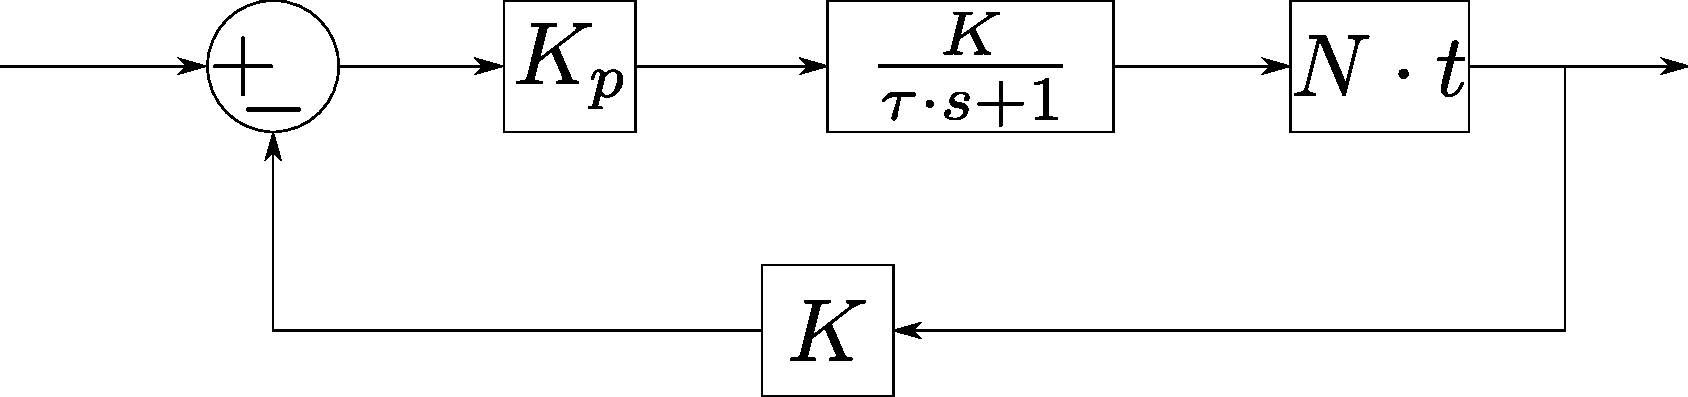
\includegraphics[scale=0.4]{figures/proportionalController.pdf}
 	\caption{Diagram of the proportional controller}
  \label{proportionalController}
\end{figure}
This gives the following closed loop transfer function:
%
\begin{flalign}
  \eq{ \frac{V_{out}}{V_{ref}} }{ \frac{\frac{ K_p \cdot K }{ K_p \cdot K + 1 } }{ \frac{ \tau }{ K_p \cdot K + 1 } \cdot s + 1} }&\label{eq:PclosedLoopTfs}
\end{flalign}
%
From this it is evident that the new system time constant is dependent on the chosen \si{K_p}. The relation is seen directly in the standard form as the coefficient of s:
%
\begin{flalign}
  \eq{ \tau_{closed} }{ \frac{ \tau }{ K_p \cdot K + 1 } }&\nonumber
\end{flalign}
%
So if \si{K_p} is chosen such that it cancels out the gain \si{K} of the plant, allowing for the linear velocity as the input, the time constant will be reduced to half, as will the gain:
\begin{flalign}
  \eq{ \frac{V_{out}}{V_{ref}} }{ \frac{\frac{ \frac{1}{K} \cdot K }{ \frac{1}{K} \cdot K + 1 } }{ \frac{ \tau }{ \frac{1}{K} \cdot K + 1 } \cdot s + 1} }&\nonumber\\
  \eq{ \frac{V_{out}}{V_{ref}} }{\frac{\frac{1}{2}}{\frac{\tau}{2} \cdot s + 1}}&\label{eq:PclosedLoop}
\end{flalign}
%
This means that the P-controller will give an output of half the input, but rise to its set-point twice as fast as the system step without control. This is tested on the vehicle and the response is as expected as seen in \appref{app:proportionalControllerTest}.
%
\subsection{P-Controller with Feed Forward}
Because of its offset the P-controller is not sufficient for reaching and so controlling the decried output velocity. However the P-controller can be improved by manipulating its set-point through use of feed forward, see \figref{proportionalControllerWithFeedforward}.
%
\begin{figure}[H]
 	\centering
 	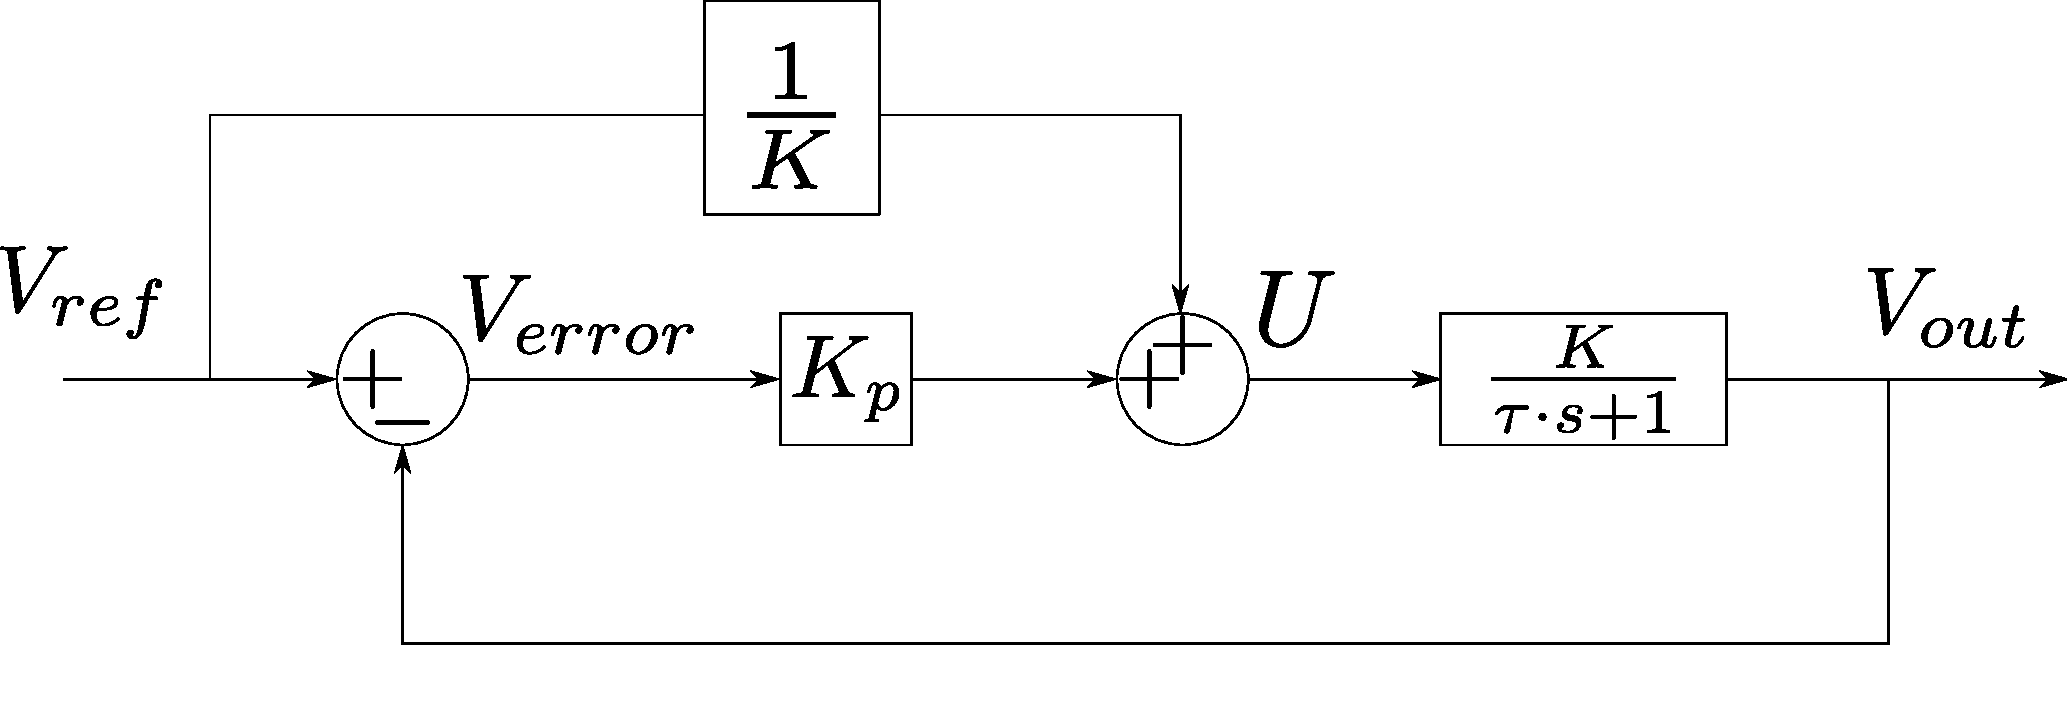
\includegraphics[scale=0.4]{figures/proportionalControllerWithFeedforward.pdf}
 	\caption{Diagram of the proportional controller with feedforward}
 	\label{proportionalControllerWithFeedforward}
\end{figure}
%
In this design the set-point is changed by forward feeding the desired value of the output \si{V_{ref}} to the input of the plant, summing up with the error fed through the P-controller. The gain on the feed forward makes sure that the value of \si{V_{ref}} is in the same unit as the signal going into the plant, here in volts, \si{U}. Since the system gain \si{K} converts volts into linear velocity, the gain in the forward feed is set to \si{\frac{1}{K}}, which yields the following closed loop transfer function:
%
\begin{flalign}
  \eq{ \frac{V_{out} }{V_{ref}} }{ \frac{\frac{K\cdot \frac{1}{K}+K\cdot K_p}{1+K \cdot K_p}}{\frac{\tau}{1+K\cdot K_p}\cdot s + 1 } }&\nonumber
\end{flalign}
%
If the \si{K_p} value again is selected to cancel out the system gain, allowing for velocity directly on the controller input, the following emerges from the closed loop transfer function:
%
\begin{flalign}
  \eq{ \frac{V_{out} }{V_{ref}} }{ \frac{\frac{K\cdot \frac{1}{K}+K\cdot \frac{1}{K}}{1+K \cdot \frac{1}{K}}}{\frac{\tau}{1+K\cdot \frac{1}{K}}\cdot s + 1 } }&\nonumber\\
  \eq{ \frac{V_{out} }{V_{ref}} }{ \frac{1}{\frac{\tau}{2} \cdot s + 1} }&\nonumber
\end{flalign}
%
If this is compared to the resulting closed loop transfer function for the original P-controller, \eqref{eq:PclosedLoop}, it is immediately obvious that the gain-problem has been solved. Notice that the time constant of the closed loop remains half of that of the plant. So by using the forward feed to place the set-point of the controller, P-control suddenly becomes a viable option for controlling the velocity. This is tested on the vehicle and the response is as expected as seen in \appref{app:proportionalControllerTest}.

If however the P-controller with feed forward is tested with an added disturbance, for instance a adding friction when breaking, the forward feed no longer compensates. The set-point compensation origins at the input of the controller, so when a disturbance is imposes on the system, the gain of the plant suddenly changes, and this cannot be accounted for with this feed forward P-controller. The effect is demonstrated in \figref{feedForwardHillOffset}\todo{make this test, and insert picture}, where the controller was tested on a hill.
%
\subsection{PI-Controller}
To attack the new offset-problem caused by changes in the system gain when disturbances enter the system, a proportional integral controller is the next natural choice. The reason for choosing a PI-controller is because the I-component integrates over the error. This component therefore increases or decreases over time, and so has an adaptive effect on the system. The design is outlined in \figref{proportionalIntegratorController}
%
\begin{figure}[H]
 	\centering
 	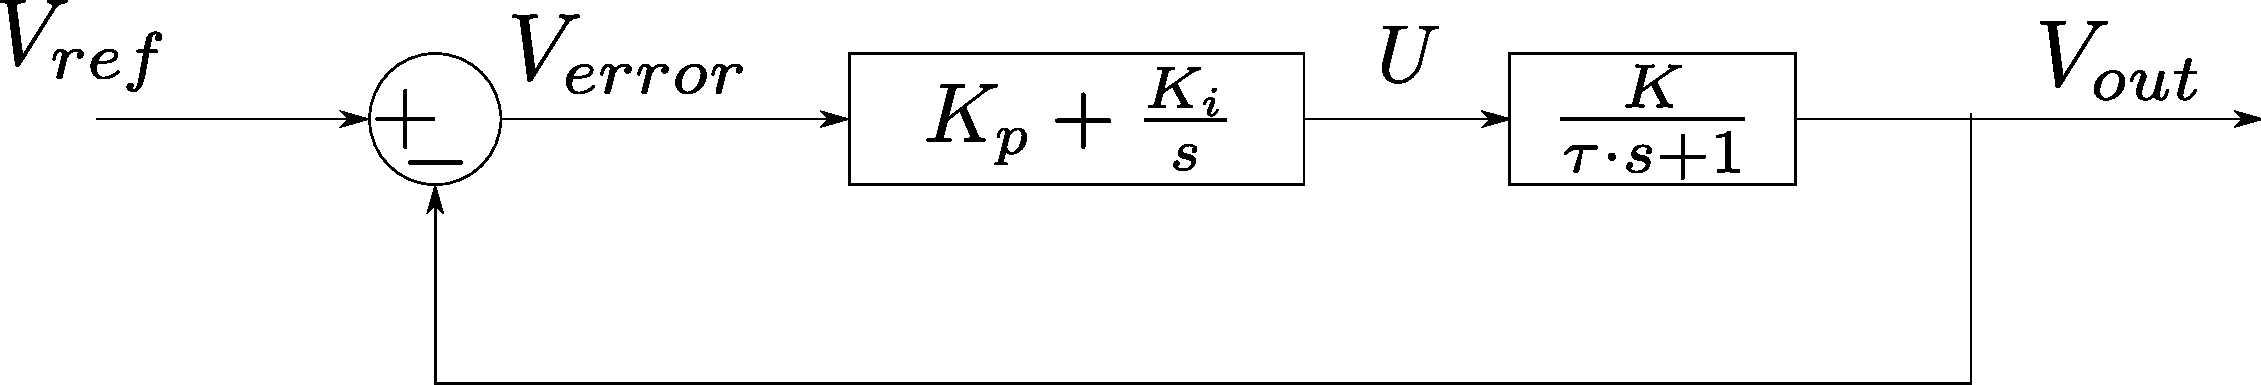
\includegraphics[scale=0.4]{figures/proportionalIntegratorController.pdf}
 	\caption{Diagram of the proportional integral controller}
 	\label{proportionalIntegratorController}
\end{figure}
%
The standard equation for a PI-controller is given and can be rewritten as:
%
\begin{flalign}
  \eq{K_p\cdot(1+ \frac{1}{T_i\cdot s})}{K_p \cdot \frac{T_i \cdot s + 1}{T_i \cdot s}}&\nonumber
\end{flalign}
%
Where \si{T_i} is the time constant of the integrator. Now if the time constant of the integrator is matched to the time constant of the plant, that is \si{T_i = \tau}, the following emerges from the closed loop transfer function:
%
\begin{flalign}
  \eq{\frac{V_{out} }{V_{ref}}}{\frac{K_p \cdot \frac{\tau \cdot s + 1}{\tau \cdot s} \cdot \frac{K}{\tau \cdot s + 1 }}{1 + K_p \cdot \frac{\tau \cdot s + 1}{\tau \cdot s} \cdot \frac{K}{\tau \cdot s + 1 }}}  \ \ \Leftrightarrow  \ \ 
  \si{\frac{V_{out} }{V_{ref}} = \frac{K_p \cdot \frac{K}{\tau \cdot s}}{1 + K_p \cdot \frac{K}{\tau \cdot s} }}&\nonumber
\end{flalign}
%
Inserting \si{K_p = \frac{1}{K}}, yields the following:
%
\begin{flalign}
  \eq{\frac{V_{out} }{V_{ref}}}{\frac{\frac{1}{K} \cdot \frac{K}{\tau \cdot s}}{1 + \frac{1}{K} \cdot \frac{K}{\tau \cdot s} }} \ \ \Leftrightarrow  \ \  \si{\frac{V_{out} }{V_{ref}} = \frac{\frac{1}{\tau \cdot s}}{1 + \frac{1}{\tau \cdot s} }} \ \ \Leftrightarrow  \ \  \si{\frac{V_{out} }{V_{ref}} = \frac{1}{\tau \cdot s + 1}}&\nonumber
\end{flalign}
%
This is equivalent to the plant but with a gain of 1 instead of K, which is desirable, and so also the reason for inserting \si{K_p = \frac{1}{K}}.
Now to determine \si{K_i}, the original equation for a PI-controller is evaluated:
%
\begin{flalign}
  \si{K_p + K_i\cdot \frac{1}{s}} &= \si{K_p\cdot(1+ \frac{1}{T_i\cdot s}) \ \ \Rightarrow \ \ K_i\cdot \frac{1}{s} = \frac{K_p}{T_i\cdot s} \ \ \Rightarrow \ \ K_i = \frac{K_P}{T_i} \ \ \Rightarrow \ \ K_i = \frac{K_p}{\tau}}&\nonumber
\end{flalign}
%
This concludes the PI-controller design.\todo{insert numbers maybe? Also write more in the "tail"}

\subsection{Comparison of the Controllers}
On \figref{fig:ControllerSteps} the different controller designs are simulated being subjected to a velocity step. For comparison the plant is subjected to a voltage step calculated from a velocity and the gain of the plant.
%
\begin{figure}[H]
 	\centering
 	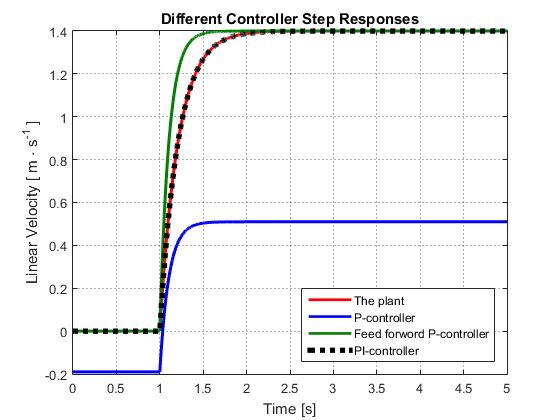
\includegraphics[width=\textwidth]{figures/ControllerSteps}
 	\caption{Diagram of the proportional controller}
 	\label{fig:ControllerSteps}
 \end{figure}
%
The first thing to notice on \figref{fig:ControllerSteps}, is the inadequacy of the P-controller, given by its steady state error. The feed forward P-controller however, solving this problem, seems like a very good solution if consulting only its step response. As discussed, a problem arises when introducing a disturbance, as seen in \figref{feedForwardHillOffset}. The last discussed option is the PI-controller, which places itself right on top of the step response of the plant when having a gain of 1, which is by design. The difference between the plant with a scaled input to obtain a gain of 1, compared to the PI-controller lies in the feedback along with the adaptive gain emerging from the I-component. This becomes clear when investigating the open loop rather than the closed loop transfer function:
%
\begin{flalign}
  V_{error}(s) \cdot \frac{(K_p \cdot \frac{K_i}{s}) \cdot K}{\tau \cdot s + 1}
  \left.\rule{0cm}{1cm}\right\vert\rule{0cm}{.7cm}_{\substack{K_p = \frac{1}{K} \\ \rule{0cm}{.1cm}\\ K_i = \frac{K_p}{\tau}}}
  &\ \ \Rightarrow \ \
  V_{error}(s) \cdot \frac{1}{\tau \cdot s}
  \ \ \xRightarrow{\mathcal{L^{\si{-1}}}} \ \
  \frac{1}{\tau} \cdot \int_{0}^{t} V_{error}(\tau_i) \ d \tau_i &\nonumber
\end{flalign}
%
\hspace{6mm} Where:\\
\begin{tabular}{p{1cm}lll}
  & \si{\tau_i}    & is an integration variable&\\
  & \si{V_{error}} & is the error from \si{V_{ref}-V_{out}}, see \figref{proportionalIntegratorController}&
\end{tabular}

This shows how the integral component of the controller integrates over the error from the reference to the output over time.

On \figref{fig:PIcontrollerStepRealVsSim} a step response of an implemented PI-controller is shown in comparison with the simulated step response with PI-controller.
%
\begin{figure}[H]
 	\centering
 	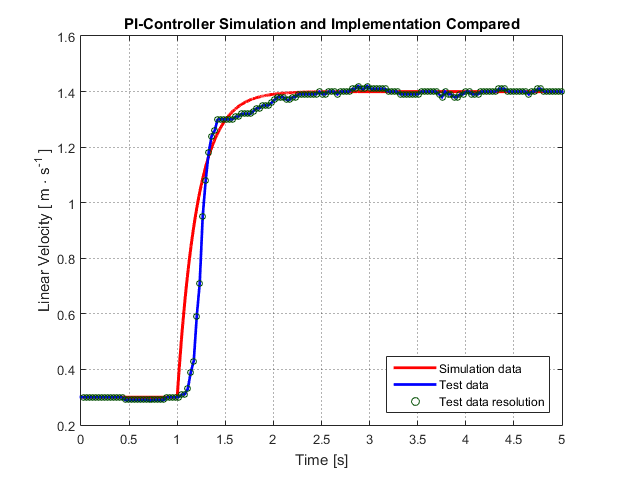
\includegraphics[width=\textwidth]{figures/PIcontrollerStepRealVsSim}
 	\caption{Diagram of the proportional controller}
 	\label{fig:PIcontrollerStepRealVsSim}
\end{figure}
%
The difference between the two responses at the bottom of the graph might be partially due to the fact that the vehicle is a \si{2^{nd}} order system. The approximation to a \si{1^{st}} order model is however not to be discarded. The design still delivers a response relatively close to the simulation, and as seen from \chapref{cha:AcceptTest}, the PI-controller fulfills the requirements set for the system's velocity controller.

\begin{figure}[H]
 	\centering
 	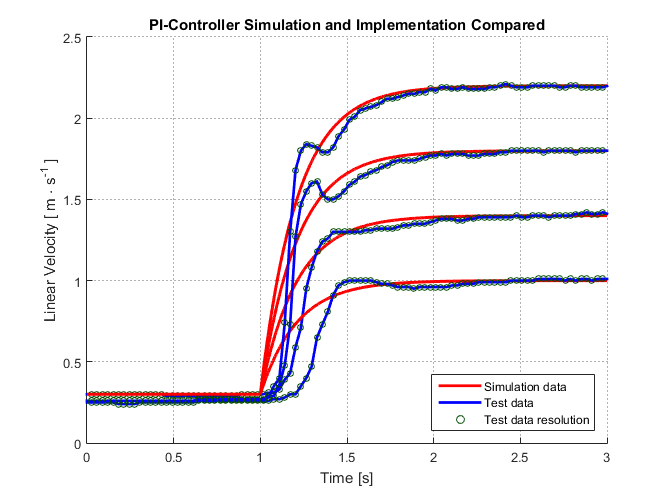
\includegraphics[width=\textwidth]{figures/multiStepPI}
 	\caption{Diagram of the proportional controller}
 	\label{fig:multiStepPI}
\end{figure}

\begin{figure}[H]
 	\centering
 	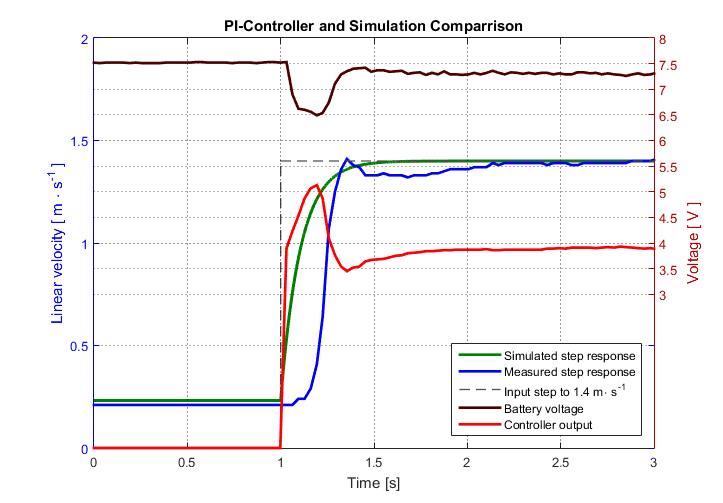
\includegraphics[width=\textwidth]{figures/CalculatedPI}
 	\caption{Diagram of the proportional controller}
 	\label{fig:CalculatedPI}
\end{figure}

\begin{figure}[H]
 	\centering
 	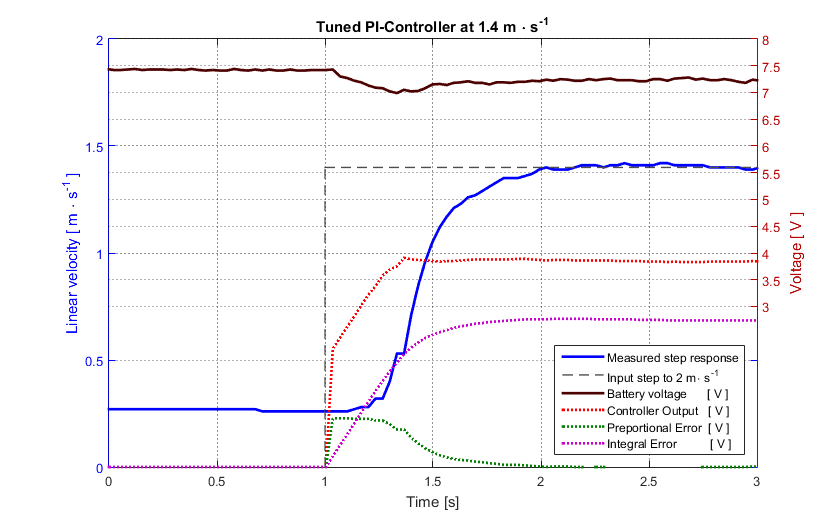
\includegraphics[width=\textwidth]{figures/TunedPI}
 	\caption{Diagram of the proportional controller}
 	\label{fig:TunedPI}
\end{figure}

